\chapter{Perception and Sensing in Robotics: Sensors and Algorithms}\label{ch:perceptionandsensing}
In this chapter we will talk about perception in industrial settings, focusing the attention on the tools, e.g. sensors and software, and the techniques used to solve industrial problems such as Random Bin Picking (RBP) and Pick\&Place (PPT) of objects. In the end we will focus also on the state of the art software libraries that nowadays are commonly used and tested in the industrial settings.

\section{Robotics in Industry}\label{sec:roboticsinindustry}
Over the years, industry has been one of the most active sector where robots and automated systems spread and diffused without limits. This is basically due to the fact that robots can easily complete tasks that humans are not capable at all, both for physical and technical failings. Robots are capable of compute the same operation multiple times without loosing any kind of accuracy and precision, they are repetitive, fast, and very well suited for industrial application, where most of the time being fast and accurate are two central points of the productive chain.

Manufacturing is one of the industrial sectors that saw the robotics ``era'' growing faster than elsewhere. Into the factories, robots are involved in every ring of the productive chain, from heavy loads handling to precise and accurate placing, from iron and metal soldering to small part assembly. The higher accuracy and velocity that robots can reach, with so high levels of repeatability and precision, brought robots, manipulators particular, at the top level of the industrial necessities.

\begin{figure}
    \centering
    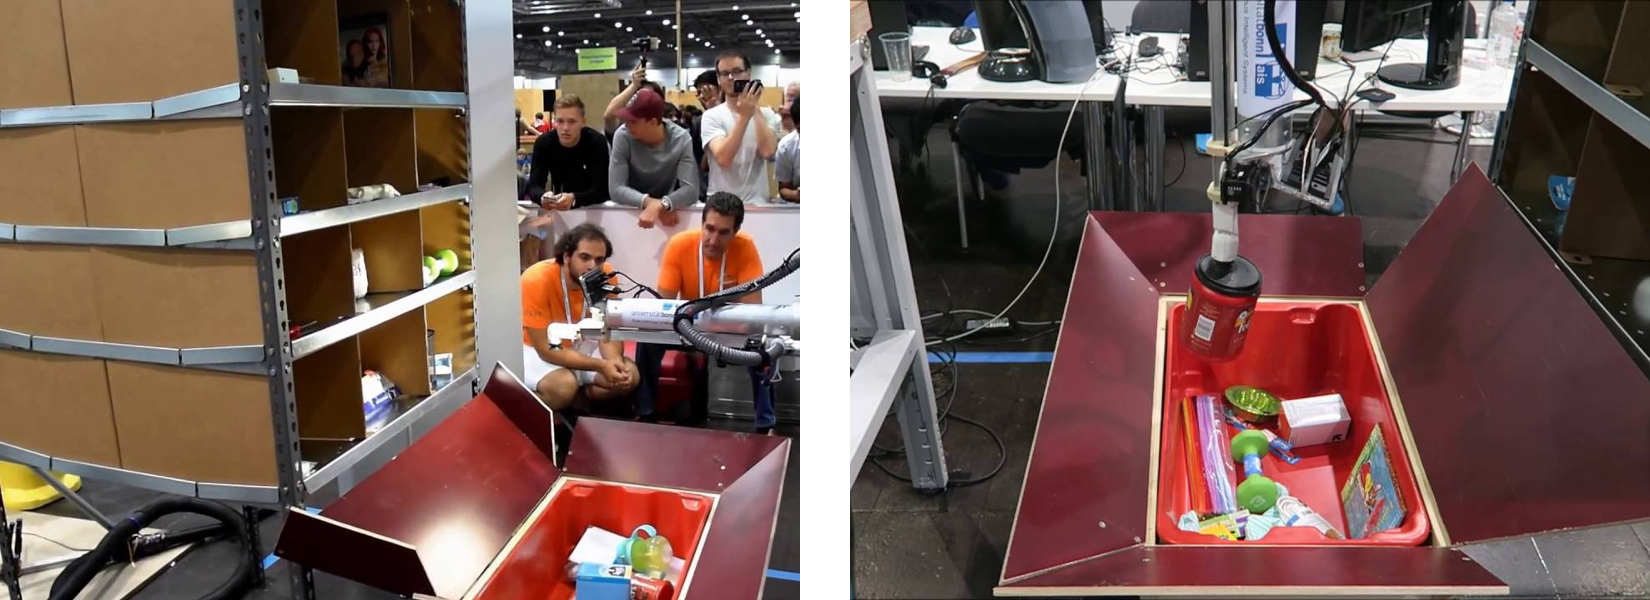
\includegraphics[width=0.8\textwidth]{figures/1_perception_and_sensing_in_robotics/amazon_picking_ch}
    \caption{\textbf{Amazon Picking Challenge example scenario.} In the images, the team is trying to detect and grasp objects from the red bin on the bottom, and place them on the shelf.} 
    \label{fig:amazon_picking_ch}
\end{figure}

The importance of robots in the industrial sector is supported also by big companies, such as Amazon, Google and others, that in the last years demonstrated high interests in investing and developing their technologies in order to improve their performance and business. One particular example of how big companies invest in robotics is the Amazon Picking Challenge competition proposed the first time at the International Conference on Intelligent Robots and Systems (IROS) in 2015 by the Amazon Robotics division\footnote{https://www.amazonrobotics.com}. This competition is thought to enhance and improve the research in the robotic manipulation, focusing the attention in grasping from random and highly cluttered environments, such as warehouse shelves or bins full of irregular and messy objects. In Figure \ref{fig:amazon_picking_ch} there are some examples of what are the typical scenarios where the teams that participate to this kind of events have to compete.

\subsection{Random Bin Picking (RBP)}\label{subsec:binpicking}
Monotonous tasks such as unloading a bin one part at a time into a machine, bulk parts sorting, and order fulfillment are labor-intensive, moreover they can even be dangerous if the parts or operations are heavy, sharp and they change position every time one object is moved away. For years, bin picking robots have been tackling these tedious jobs, but there are still so many applications to be realized.

While more capable than ever, robotic bin picking still has its limitations. It is all matter of accuracy. While robots are applauded for their repeatability, random bin picking requires accuracy in the face of chaos. The robot has to locate a part in free space, in an unstructured environment where the parts keep shifting positions and orientations every time a part is removed from the bin. That requires a delicate balance between robotic dexterity, machine vision, software, computing power to crunch all the data in real time, and a grasping solution to extract the parts from the bin. All those highly technical challenges give to RBP higher complexity and difficulty.

First of all, a brief introduction to all the kinds of Bin Picking must be given. There are three main types of bin picking: structured, semi-structured, and random bin picking. Each presents an increasing level of application complexity, cost and cycle time:

\begin{itemize}
	\item \textbf{Structured}. Parts are positioned or stacked in the bin in an organized, predictable pattern, so they can be easily imaged and picked.
	\item \textbf{Semi-Structured}. Parts are positioned in the bin with some organization and predictability to help aid imaging and picking.
	\item \textbf{Random}. Parts are in totally random positions in a bin, including different orientations, overlapping, and even entangled, further complicating the imaging and picking functions.
\end{itemize}

From now on we will concentrate on Random Bin Picking, that is the main area in which we tested our work, moreover, the RAW dataset that will be presented later in this thesis and all the developed tools, have been thought for such robotic task in particular.

\begin{figure}
    \centering
    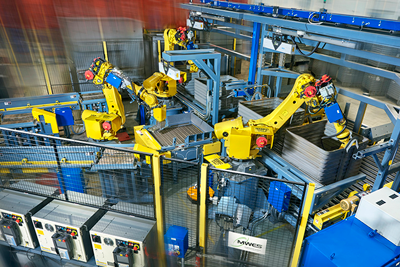
\includegraphics[width=0.8\textwidth]{figures/1_perception_and_sensing_in_robotics/rbp_example}
    \caption{\textbf{Random Bin Picking Example.} Robotic random bin picking and part loading system uses 3D vision guided robots with magnetic grippers to locate and pick parts for a heat treating operation.} 
    \label{fig:rbp_example}
\end{figure}

\begin{figure}
    \centering
    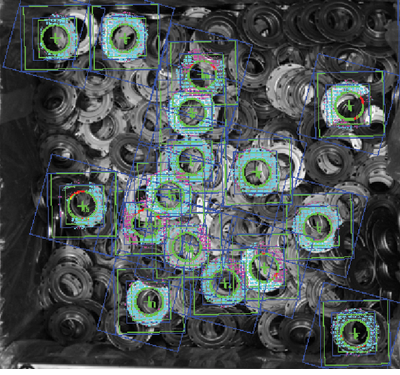
\includegraphics[width=0.5\textwidth]{figures/1_perception_and_sensing_in_robotics/cluttered_env_rbp}
    \caption{\textbf{Machine vision algorithm execution example in RBP task.} Here, a 3D area sensor is performing localization and recognition of random parts in a bin. Thanks to this technology, the robot should be capable of planning its next pick in the clutter.} 
    \label{fig:cluttered_env_rbp}
\end{figure}

An example of a robotic system performing random bin picking operation is depicted in Figure \ref{fig:rbp_example}. In this kind of scenarios, the role of vision is crucial. Vision systems must be capable of recognize, detect and localize the parts with extremely high accuracy. Typical scenarios are like the one in Figure \ref{fig:cluttered_env_rbp}, it's clearly visible how the environment is cluttered, all the parts are randomly spread inside the bin, and the task of recognizing and localizing the next part to be picked, it's extremely difficult. 

\subsection{Pick\&Place Tasks (PPT)}\label{subsec:pickandplace}
More generic, but with the same importance as the previous one, Pick\&Place (PPT) task is another interesting robotic application in which vision and perception play an important role. Differently from the aforementioned Bin Picking applications, in Pick\&Place scenarios, camera setup is not always fixed, they are mounted on the robotic arm, and the arm itself is not said to be fixed on the ground. 

A clear example of Pick\&Place scenario is the RoboCup@Work Competition, where the robotic arm that performs pick and drop operations with the objects, is actually mounted on a mobile platform that operates in a more large environment.

\section{3D Reconstruction}\label{sec:3dreconstruction}
To do ...

\section{Object Detection}\label{sec:objectdetection}
To do ...

\section{State of the art Software Libraries in Industry}\label{sec:industrylibraries}
Machine Vision is one of the most active area in industrial settings. Over the past years, many software companies and Open Source communities have dedicated lot of effort in developing robust and effective techniques and algorithms in order to assist industrial realities, such as companies and start ups, in performing computer vision assisted tasks, e.g. random bin picking, Pick\&Place tasks and so on.

In the following subsection a list of tools and libraries will be introduced, focusing mainly on the MVTec's Halcon Libraries, which are the one that we used in the experiment phase of this work. 

\subsection{Halcon Libraries}\label{subsec:halconlibs}
Halcon\footnote{http://www.mvtec.com/products/halcon/}, from MVTec, is a set of commercial software developed and sold explicitly for industrial settings. Over the past 5 years it has become the state of the art in machine vision for industrial tasks. It serves all industries with an extensive library of more than 1600 operators for blob analysis, morphology, matching, measuring, identification, and 3D vision, to name just a few.

The full library can be accessed from common programming languages like C, C++, C\#, Visual Basic .NET, and Delphi. In particular, our tests have been developed using the C++ APIs. In the following chapters we will test this standard Machine Vision approaches over the RAW and T-Less datasets, and compare them with completely different approaches such as Deep Learning CNNs for object localization and recognition.

\begin{figure}
    \centering
    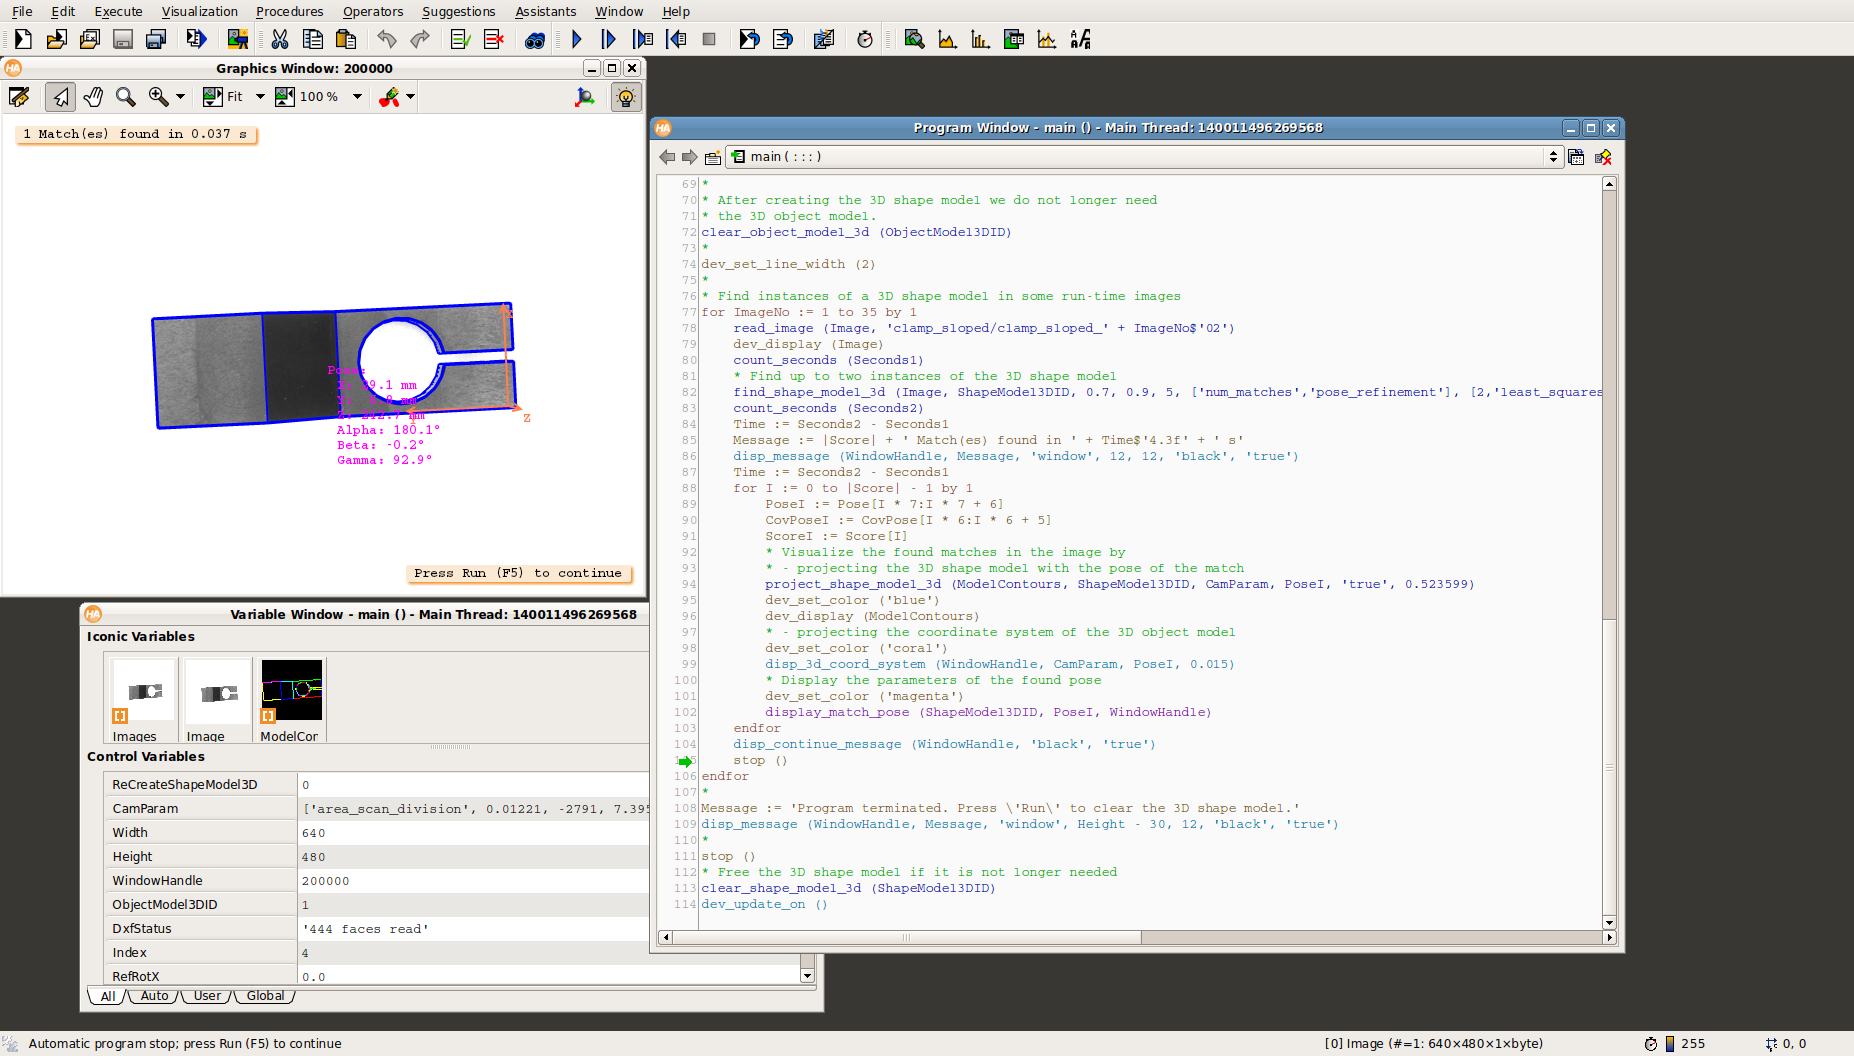
\includegraphics[width=0.8\textwidth]{figures/1_perception_and_sensing_in_robotics/hdevelop_gui_example}
    \caption{\textbf{Hdevelop GUI example.} An example of using the Hdevelop software from the Halcon Libraries. In particular here we are performing an object detection and localization task.} 
    \label{fig:hdevelop_example}
\end{figure}

The Halcon Library has also an interactive and friendly GUI, provided in order to facilitate the interfacing with the low level software APIs. The aforementioned software tool is called HDevelop, and an example of its usage and graphical interface is depicted in Figure \ref{fig:hdevelop_example}.

As anticipated, this software library is under commercial license, and our distribution has been sold to La Sapienza University of Rome that can use it for research and other non-commercial purposes. 

\begin{figure}
    \centering
    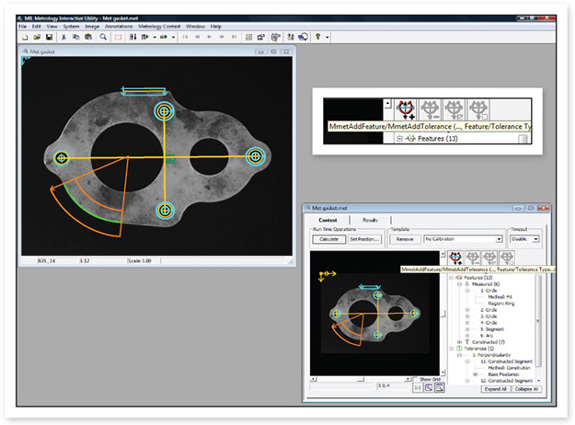
\includegraphics[width=0.8\textwidth]{figures/1_perception_and_sensing_in_robotics/mil_gui_example}
    \caption{\textbf{MIL GUI example.} The graphical user interface of the Matrox Imaging Library.} 
    \label{fig:mil_example}
\end{figure}

\subsection{Matrox Imaging Library (MIL)}\label{subsec:mil}
Another important software library that needs to be mentioned is the Matrox Imaging Library\footnote{https://www.matrox.com/imaging/en/products/software/mil/} (MIL). MIL is a complete collection of software tools for developing machine vision in lots of different scenarios, it is not restricted to the industrial one such as for the previously mentioned Halcon Libraries, but it covers also medical images applications and many others.

MIL includes also a graphic user interface for fast developing and prototyping of solutions. An example of this GUI is depicted in Figure \ref{fig:mil_example}.

This library is not part of the tests and examples performed during this work.